\chapter{Avaliação dos resultados do experimento}
	\section{ETAPA 1 – Display de 7 segmentos}

		Verificou-se, para todos os casos de entrada, que o valor previsto pela tabela-verdade
como saída era válido, demonstrando sucesso na implementação do experimento. Isso pode ser visualizado
tanto pela simulação, como na execução na placa.

		\begin{figure}[H]
			\centering

			\begin{subfigure}[b]{0.44\textwidth}
				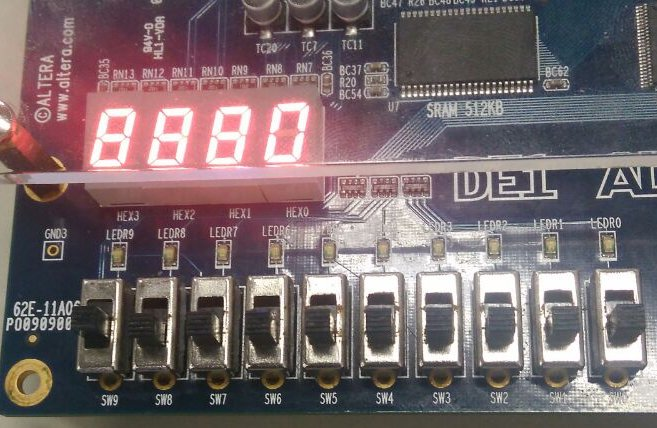
\includegraphics[width=\textwidth]{img/etapa1/0}
				\label{fig:etapa1-0}
				\caption{Número 0}
			\end{subfigure}
			~
			\begin{subfigure}[b]{0.44\textwidth}
				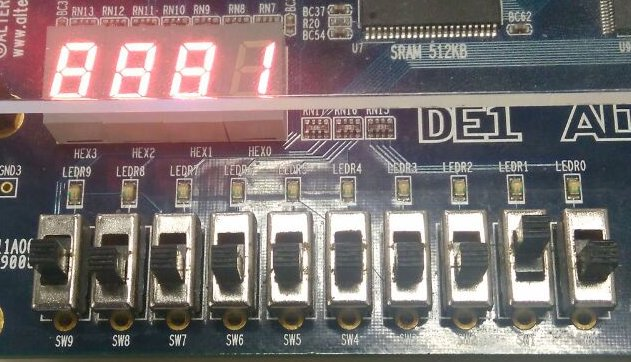
\includegraphics[width=\textwidth]{img/etapa1/1}
				\label{fig:etapa1-1}
				\caption{Número 1}
			\end{subfigure}

			\begin{subfigure}[b]{0.44\textwidth}
				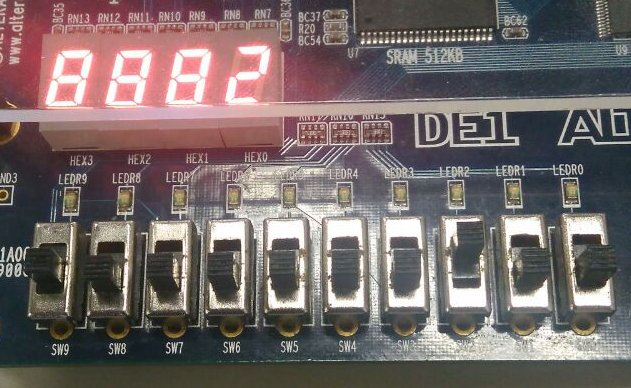
\includegraphics[width=\textwidth]{img/etapa1/2}
				\label{fig:etapa1-2}
				\caption{Número 2}
			\end{subfigure}
			~
			\begin{subfigure}[b]{0.44\textwidth}
				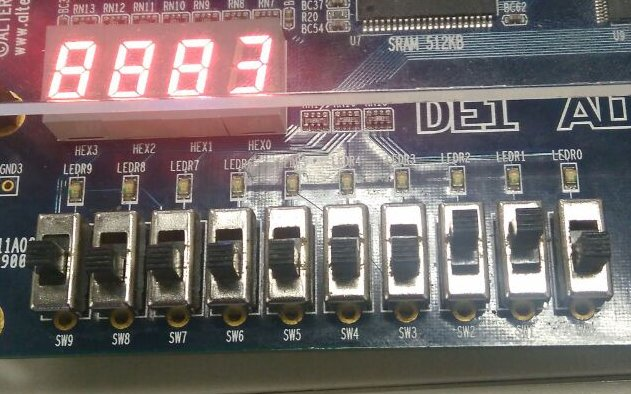
\includegraphics[width=\textwidth]{img/etapa1/3}
				\label{fig:etapa1-3}
				\caption{Número 3}
			\end{subfigure}
			\begin{subfigure}[b]{0.44\textwidth}
				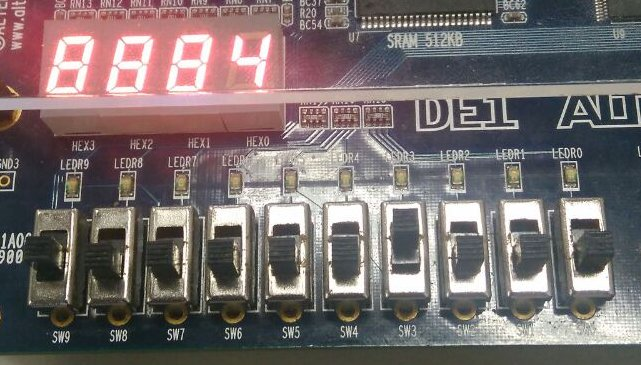
\includegraphics[width=\textwidth]{img/etapa1/4}
				\label{fig:etapa1-4}
				\caption{Número 4}
			\end{subfigure}
			~
			\begin{subfigure}[b]{0.44\textwidth}
				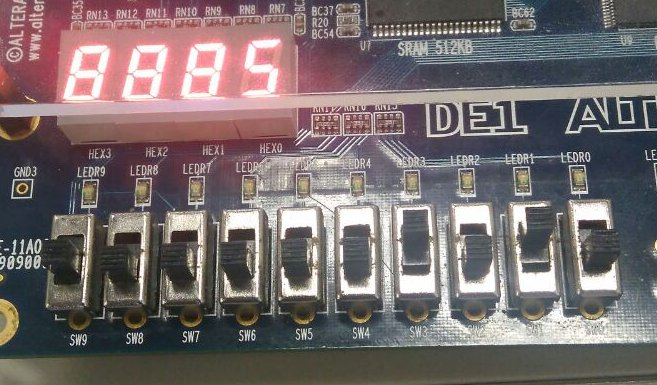
\includegraphics[width=\textwidth]{img/etapa1/5}
				\label{fig:etapa1-5}
				\caption{Número 5}
			\end{subfigure}

			\caption{Teste do circuito rodando na placa, no intervalo de 0-5.}\label{fig:estapa1Teste1}
		\end{figure}

		\begin{figure}[H]
			\centering

			\begin{subfigure}[b]{0.44\textwidth}
				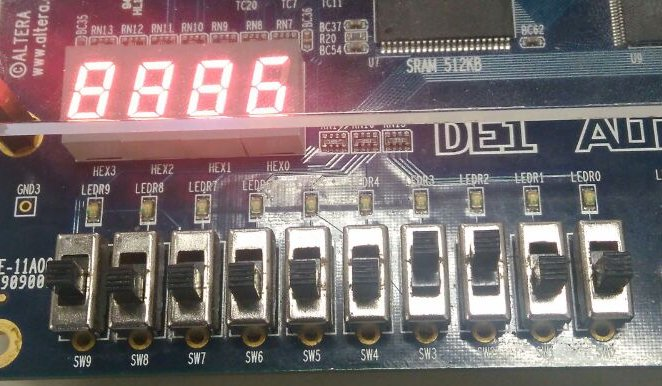
\includegraphics[width=\textwidth]{img/etapa1/6}
				\label{fig:etapa1-6}
				\caption{Número 6}
			\end{subfigure}
			~
			\begin{subfigure}[b]{0.44\textwidth}
				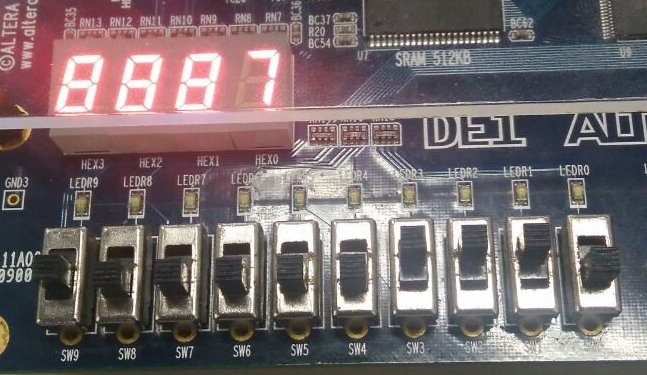
\includegraphics[width=\textwidth]{img/etapa1/7}
				\label{fig:etapa1-7}
				\caption{Número 7}
			\end{subfigure}

			\begin{subfigure}[b]{0.44\textwidth}
				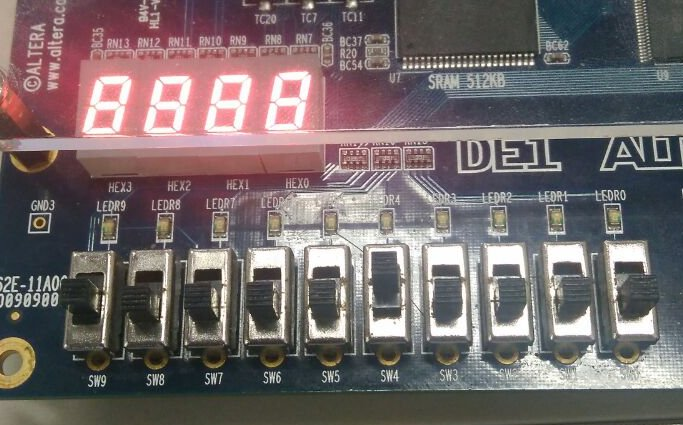
\includegraphics[width=\textwidth]{img/etapa1/8}
				\label{fig:etapa1-8}
				\caption{Número 8}
			\end{subfigure}
			~
			\begin{subfigure}[b]{0.44\textwidth}
				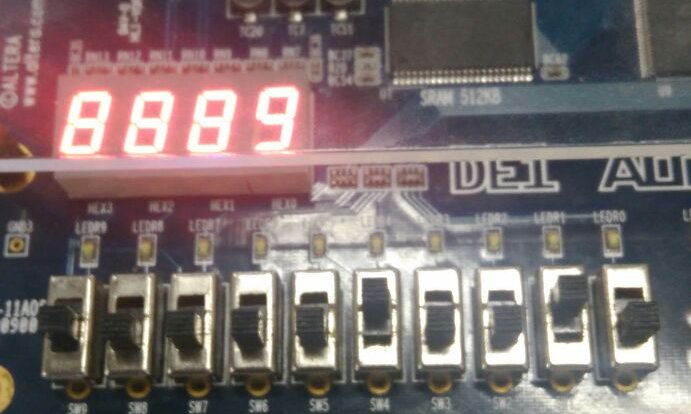
\includegraphics[width=\textwidth]{img/etapa1/9}
				\label{fig:etapa1-9}
				\caption{Número 9}
			\end{subfigure}

			\caption{Teste do circuito rodando na placa, no intervalo de 6-9.}\label{fig:estapa1Teste2}
		\end{figure}

		\begin{figure}[H]
		    \centering
			\caption{\label{fig:etapa1Simulacao}Resultado da simulação da etapa 1.}
			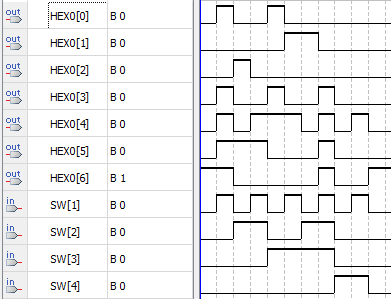
\includegraphics[width=1\textwidth]{img/SimulacaoSegmentos7}
		\end{figure}


	\section{ETAPA 2 – Meio-somador 1 bit}

	\section{ETAPA 3 – Meio-somador 4 bits}


Apresentar os resultados da simulação em software e da utilização do Kit DE1 e/ou
protoboard. Utilizar figuras, descrevê-las e discuti-las.
